\documentclass{article}
\usepackage{fancyhdr}
\usepackage{tabu}
\usepackage[bottom=1in]{geometry}
\usepackage{multirow}
\usepackage{graphicx}
\usepackage{parskip}
\usepackage{pdfpages}
\setlength{\parindent}{15pt}

%\pagestyle{fancy}

\begin{document}
%USAFA DFEC Header
	\noindent \begin{tabu} to \textwidth{l X[c] r}
	\multirow{5}{*}{
\includegraphics[width=0.75in]{DOD.jpg}} & 
	\textbf{United States Air Force Academy} &  
	\multirow{5}{*}{
\includegraphics[width=0.75in]{USAFA.png}}\\
	& \textbf{Department of Electrical and Computer Engineering} & \\
	& \tiny{USAF ACADEMY, COLORADO}\\
	\\ \\ \\
	\end{tabu}

%Start text here
	\hfill 1 Oct 2013
	\centerline{\LARGE{\textbf{Why Oxford?}}} \hspace{0pt} \\
	\centerline{\Large{Captain Ryan Silva}}
	\centerline{\large{Assistant Professor}}
	\centerline{\large{Department of Electrical and Computer Engineering}}
	\centerline{\large{United States Air Force Academy}} \hspace{0pt} \\
\indent My ultimate goal in pursuing the Oxford experience is be to bring world-class
Biomedical Engineering research opportunities to USAFA. The core academic
strengths of Oxford's Center for Affordable Healthcare Technology (OxCAHT) and
the open-source nature of their research paired with Oxford's matchless
geopolitical landscape make the University of Oxford the only English-speaking
university in the world with whom my research aspirations can be accomplished.
I believe bringing these research opportunities in biomedical engineering back
to USAFA, through a partnership with OxCAHT, will allow for generations of cadets
and faculty to draw from the immensely deep well that is research in innovative medical technology.
I also believe that I am the perfect candidate with whom you can trust to accomplish
this lofty objective.

As an award-winning project mentor for the senior capstone project
NeuMimic, funded through FalconWorks, I would bring bring OxCAHT valuable experience leading a
successful multi-disciplinary, systems-level biomedical engineering research project. I would 
come armed with valuable leadership experience paired with technical expertise in signal 
processing and embedded systems, thereby poised to become an immediate contributor;
it is important to note that the director of OxCAHT, Dr. Gari Clifford, agrees
with my assessment. Dr. Clifford, after a \emph{very} thorough Skype interview,
offered me a place on his team; in fact, he already has a project in mind for me to work on. 
The project is outlined in a signed MFR that can be found in Attachment 1
on page~\pageref{sec:prop}. The project has been scaled for appropriateness and feasibility of
completion in 3 years. I am so excited at the prospect of pursuing this project that it feels as though this opportunity was tailored to suit my strengths and interests! 
 
Based on its potential contributions to human well-being, there are few fields
that offer more inspiring opportunities for research than biomedical engineering, especially the subject areas involving medical diagnostics.
Diagnostics is a very challenging discipline as it usually involves
prohibitively expensive and immobile equipment that regularly forces patients
to travel great distances at great cost in order to access care. These traits
currently inherent to medical diagnostics regularly exclude certain
populations from receiving proper
treatment. Affected populations can range from military members operating in an
expeditionary environment to inhabitants of rural communities, especially in the developing
world. My proposed research seeks to develop solutions to the critical need for
point of care devices that are cheap, power-efficient, reliable and
transportable. The immediate impact of this research is clear: it will allow
individuals to access healthcare that otherwise would not be able. Oxford's
centuries-old geopolitical affiliations allow this type of research to progress 
at a pace unrivaled at any other university or center. This is proven by the
expectations of the program, which involve identifying a real-world diagnostic 
shortfall, creating a novel solution to fill the need as well as conducting
clinical trials all within the standard 3 year time frame necessary to 
complete the degree. There is simply no other place on earth where research of
this type can progress from idea to clinical trials within this relatively short
time frame. While it is important to emphasize that this is exciting research,
it is also important to highlight where USAFA Cadets fit in.
 
OxCAHT follows a research model based on the mission of Engineering World
Health ``to inspire and mobilize the biomedical engineering community to improve
the quality of health care in resource-poor communities of the developing
world" (www.oxcaht.org) . The ``mobilization" aspect of the above mission
statement effectively created a desire within the Biomedical Engineering 
community to take the handcuffs off traditional academic research. This has
been accomplished by embracing an open-source paradigm for conducting research.
The result of this paradigm is the creation of a ``Wikipedia" for biomedical
engineering research called PhysioNet, which is an open-source repository of
academic endeavors to which anyone may contribute. This repository is
predominately comprised of computer source code and raw diagnostic data but
also contains hardware schematics, mechanical drawings and other documentation
of studies, technologies, and data contributing to the field of biomedical
engineering. The open-source nature of this research is particularly
interesting when incorporated with the research climate of USAFA.
 
Developing a research partnership between Oxford and USAFA based on open-source
technology through PhysioNet is a relatively simple process to navigate, in fact I already have.
I have garnered approvals through Col Kraus, USAFA Office of Research, and the
USAFA Judge Advocate for the research partnership I am proposing (the
approvals can be found in Attachments 2 and 3
respectively). Oxford-level research opportunities can
exist at USAFA, not as an arcane future promise, but as a detailed plan that
begins with choosing me for the Dean's Oxford Scholarship. Not only am I the
best candidate to develop and pursue these exciting research opportunities, I
am also the best candidate to bring these opportunities back to USAFA and
inspire a new generation of cadets dedicated to making tangible contributions
to the health and wellbeing of humanity.

The director of OxCAHT is in a unique situation. He is in a position to make
immense contributions to the physical health of entire populations, but he needs
help. Particularly, he needs help designing and implementing embedded solutions
to a plethora of diagnostic shortfalls. His center does an amazing job
identifying diagnostic issues in the developing world and creating advanced algorithms that use
state-of-the-art machine learning and brilliant signal processing techniques to
properly analyze diagnostics data, but what he is missing is a team of
undergraduates willing to implement the OxCAHT solutions in hardware such that
they can be tested in the field. This is where USAFA Cadets come in. My experience with 
Neumimic demonstrates that USAFA Cadets are capable of developing and implementing biomedical 
signal processing techniques because they are already doing it. I can only
imagine what USAFA Cadets could accomplish if they could leave the signal processing element
of their current research to expert researchers working for the Oxford Center 
for Affordable Healthcare Technology and focus on implementing their diagnostic 
solutions into hardware! Once a partnership is established between Oxford and USAFA,
cadets could expect to create hardware platforms that make OxCAHT's advanced processing techniques
work in real life. These devices could then be transferred back to Oxford, through Physionet,
where they will be tested and, quite possibly, administered to real patients by Oxford researchers.
What an exciting opportunity for all involved!
 
I want to state unequivocally that my assignment at USAFA has easily been the
most rewarding experience of my career. I am truly passionate about the USAFA
Mission and I believe there is no greater professional fulfillment than to see
the sheer magnitude of positive influence and inspiration an officer can have
in a cadet's life. I've found that this is accomplished through tireless
devotion in and out of the classroom. My first tour has taught me to appreciate
the immense responsibility associated with shaping and motivating America's
future leaders, and it would be a privilege and an honor to be trusted with
that responsibility again by selecting me to bring Oxford-caliber opportunities
back to USAFA as a senior military faculty member.
 
My resume clearly illustrates that I have thrived during my time in DFEC as I
have won every award the department has to give as well as garnered national
level recognition as the Great Minds in Stem Most Promising Engineer of 2013,
but there is no formal record of the 3 accolades I hold most dear: I have been
afforded the opportunity to participate in the culmination of the USAFA Mission
through administering the Oath of Office thereby commissioning 3 cadets into
Active Duty. When considering who should administer the Oath, cadets are
instructed to select the officer whose inspiration had the greatest impact on
their development and whose leadership they would most like to emulate. It is
humbling to consider that these (now) Lieutenants in the classes of 2011, 2012
and 2013 selected me to be a part of the zenith of their USAFA careers and the
arbiter that bestows upon them the prize for which they have worked so hard.
Ultimately my personal commitment to the USAFA Mission has been recognized by
my fellow faculty and endorsed by cadets, whose interests USAFA exists to
serve. Choose me for the Dean's Oxford Scholarship and the real winners are the
cadets.

Gus Jones!

\newpage
\section*{Attachment 1 \newline Approved Oxford Research Proposal}
\label{sec:prop}
\centering
\vspace{-5mm}
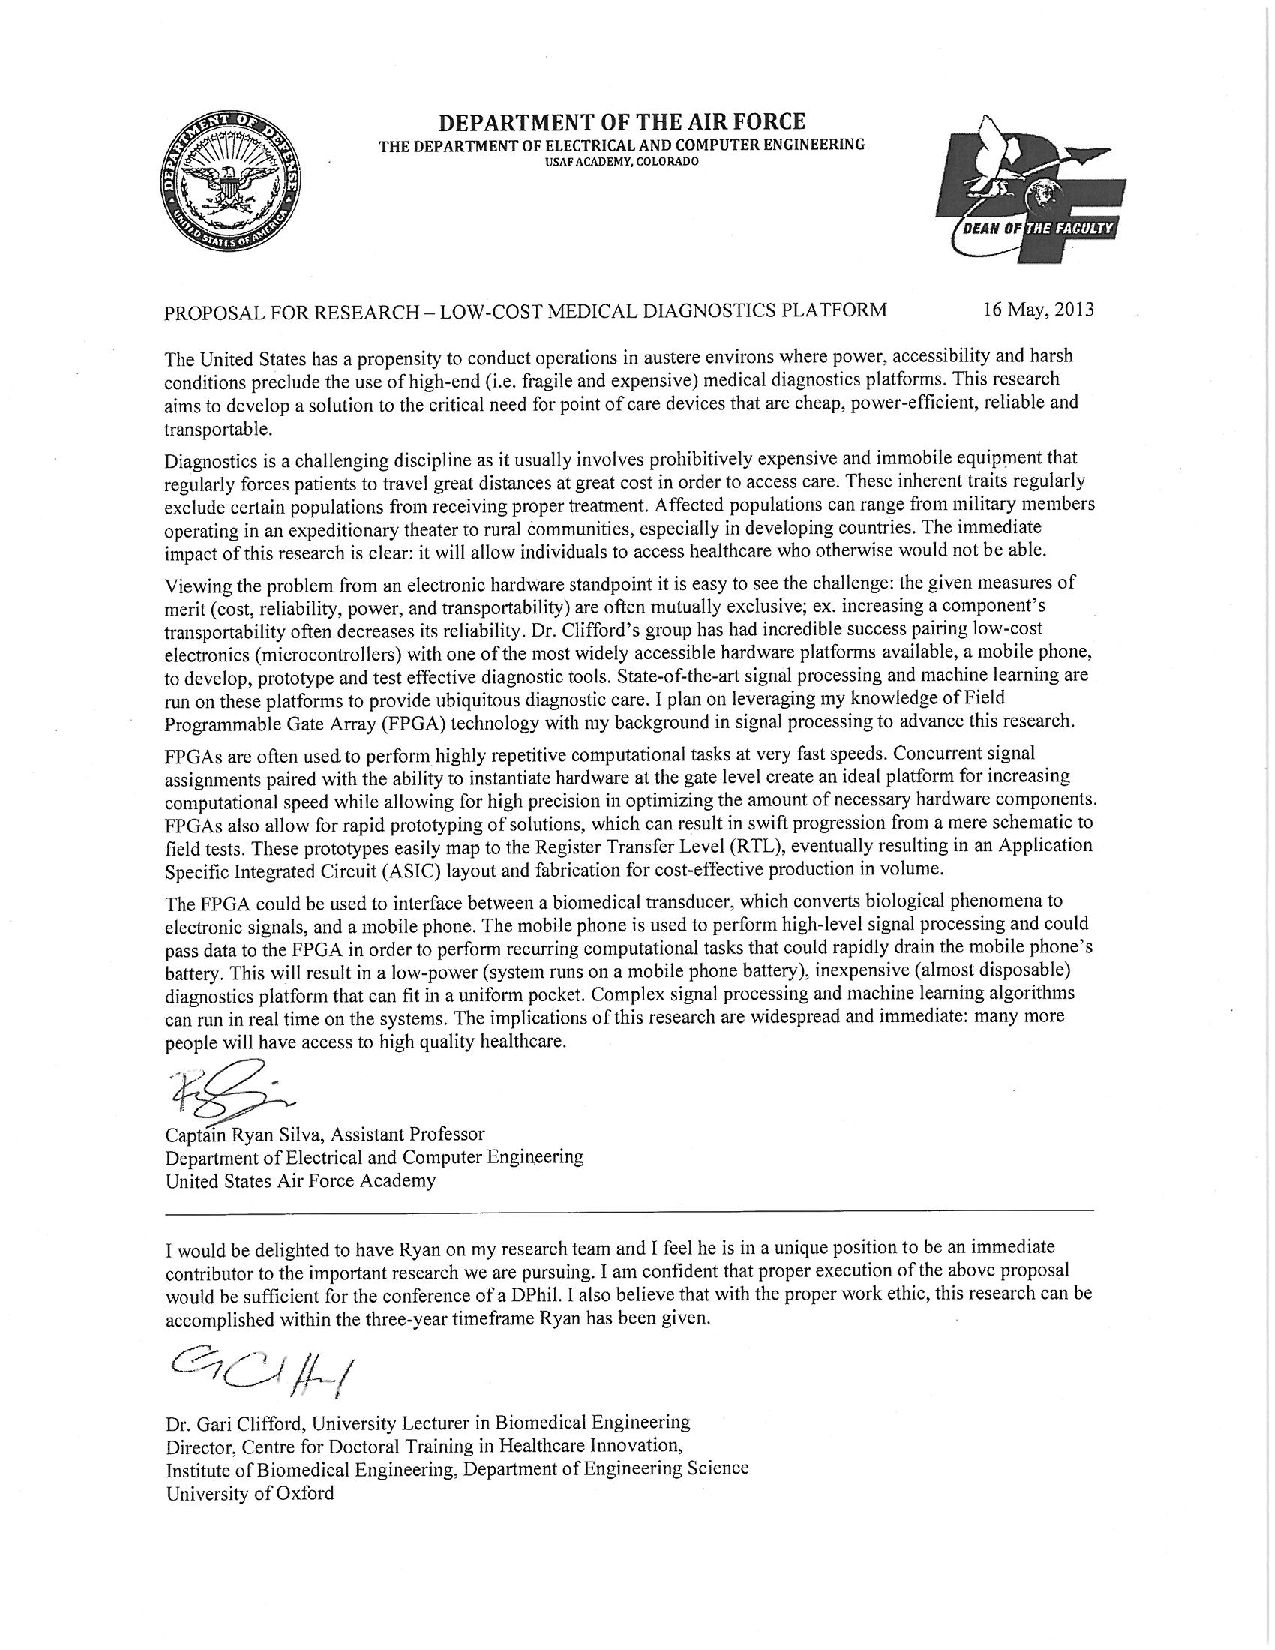
\includegraphics[scale=.85,clip=true,trim=1in .5in 1cm 0.4in]{MFR_ProposalforResearch_SilvaSIGNED.pdf}

\newpage
\section*{\raggedright Attachment 2 \newline DF Research Office Approval to Conduct Research}
\label{sec:DFER}
\centering
\vspace{-1cm}
\hspace*{-1.5cm}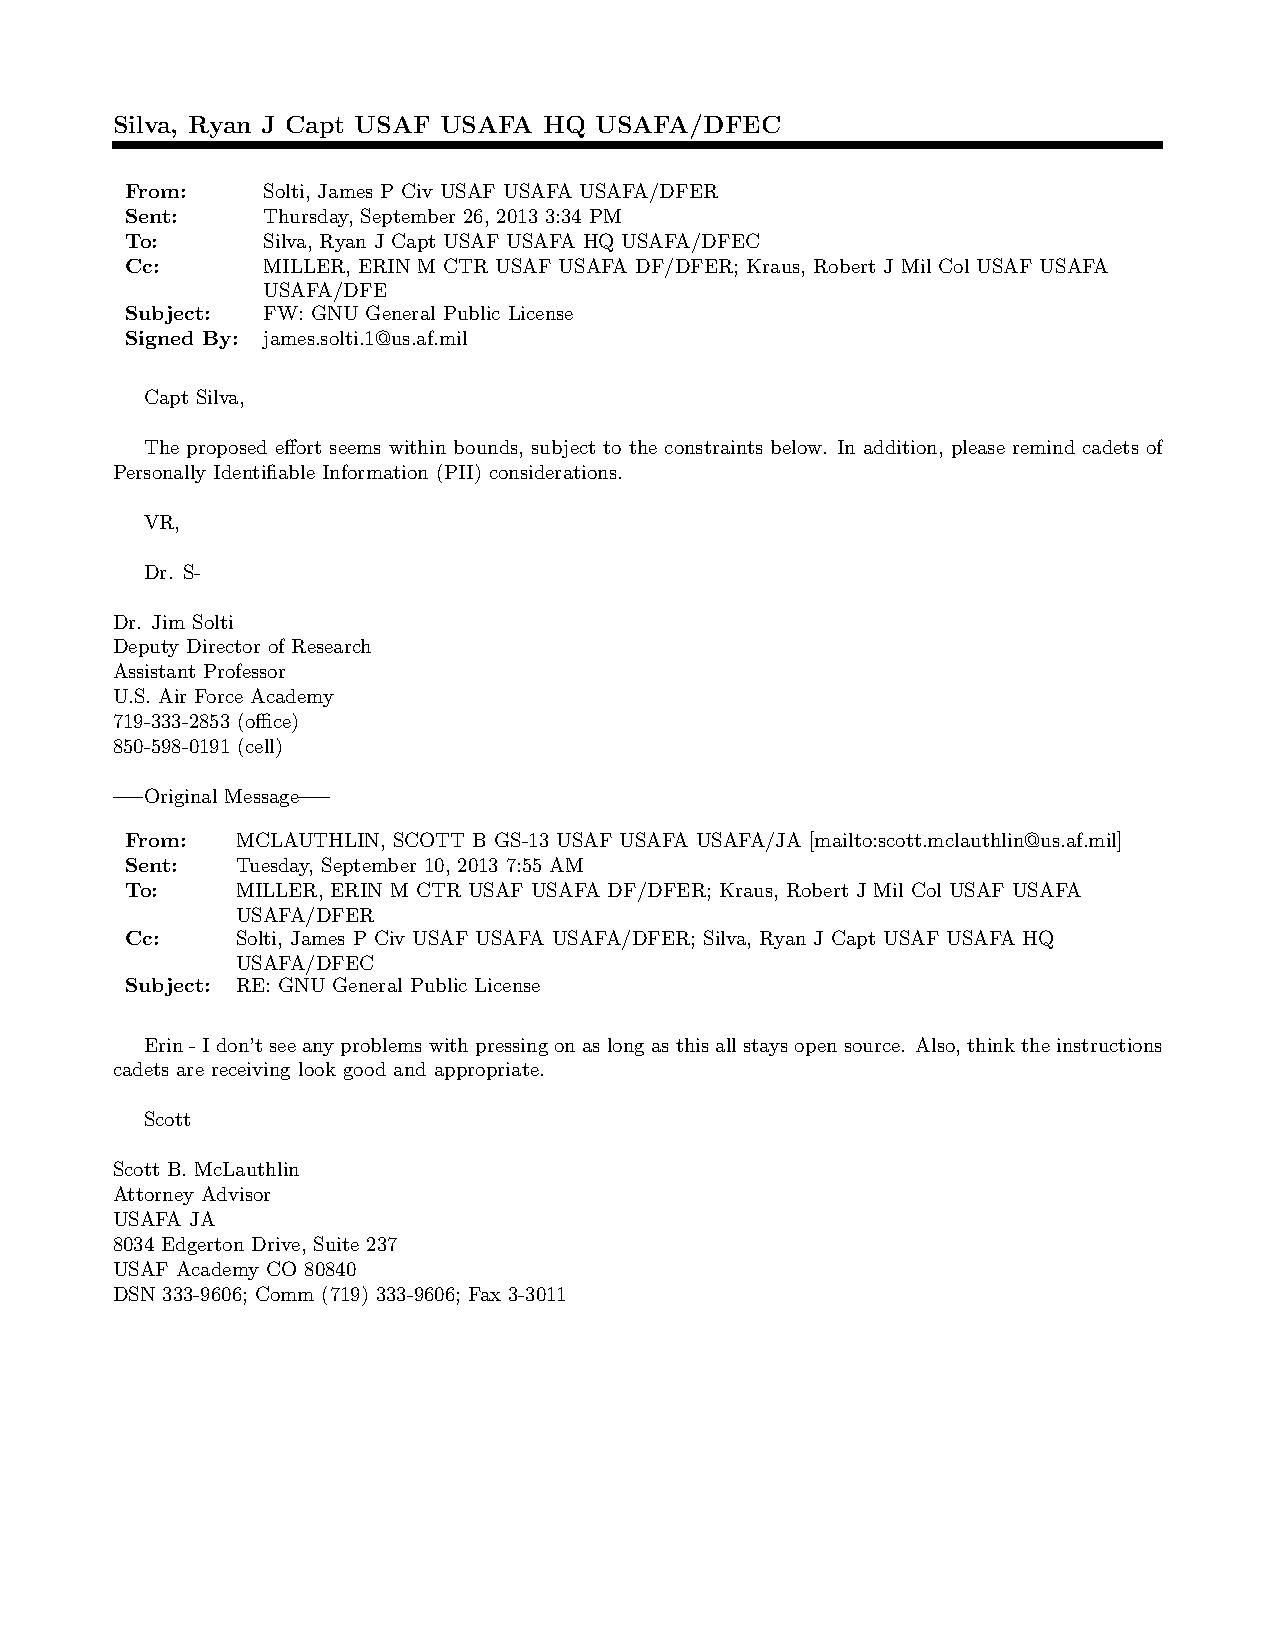
\includegraphics[scale=.85]{DFER_email.pdf}
\includepdf[pages=2-3,scale=0.85,offset=-0 -25,pagecommand={}]{DFER_email.pdf}
\newpage
\section*{\raggedright Attachment 3 \newline USAFA Judge Advocate Approval to Conduct Research}
\label{sec:JA}
\centering
\vspace{-0.1cm}
\hspace*{-1.5cm}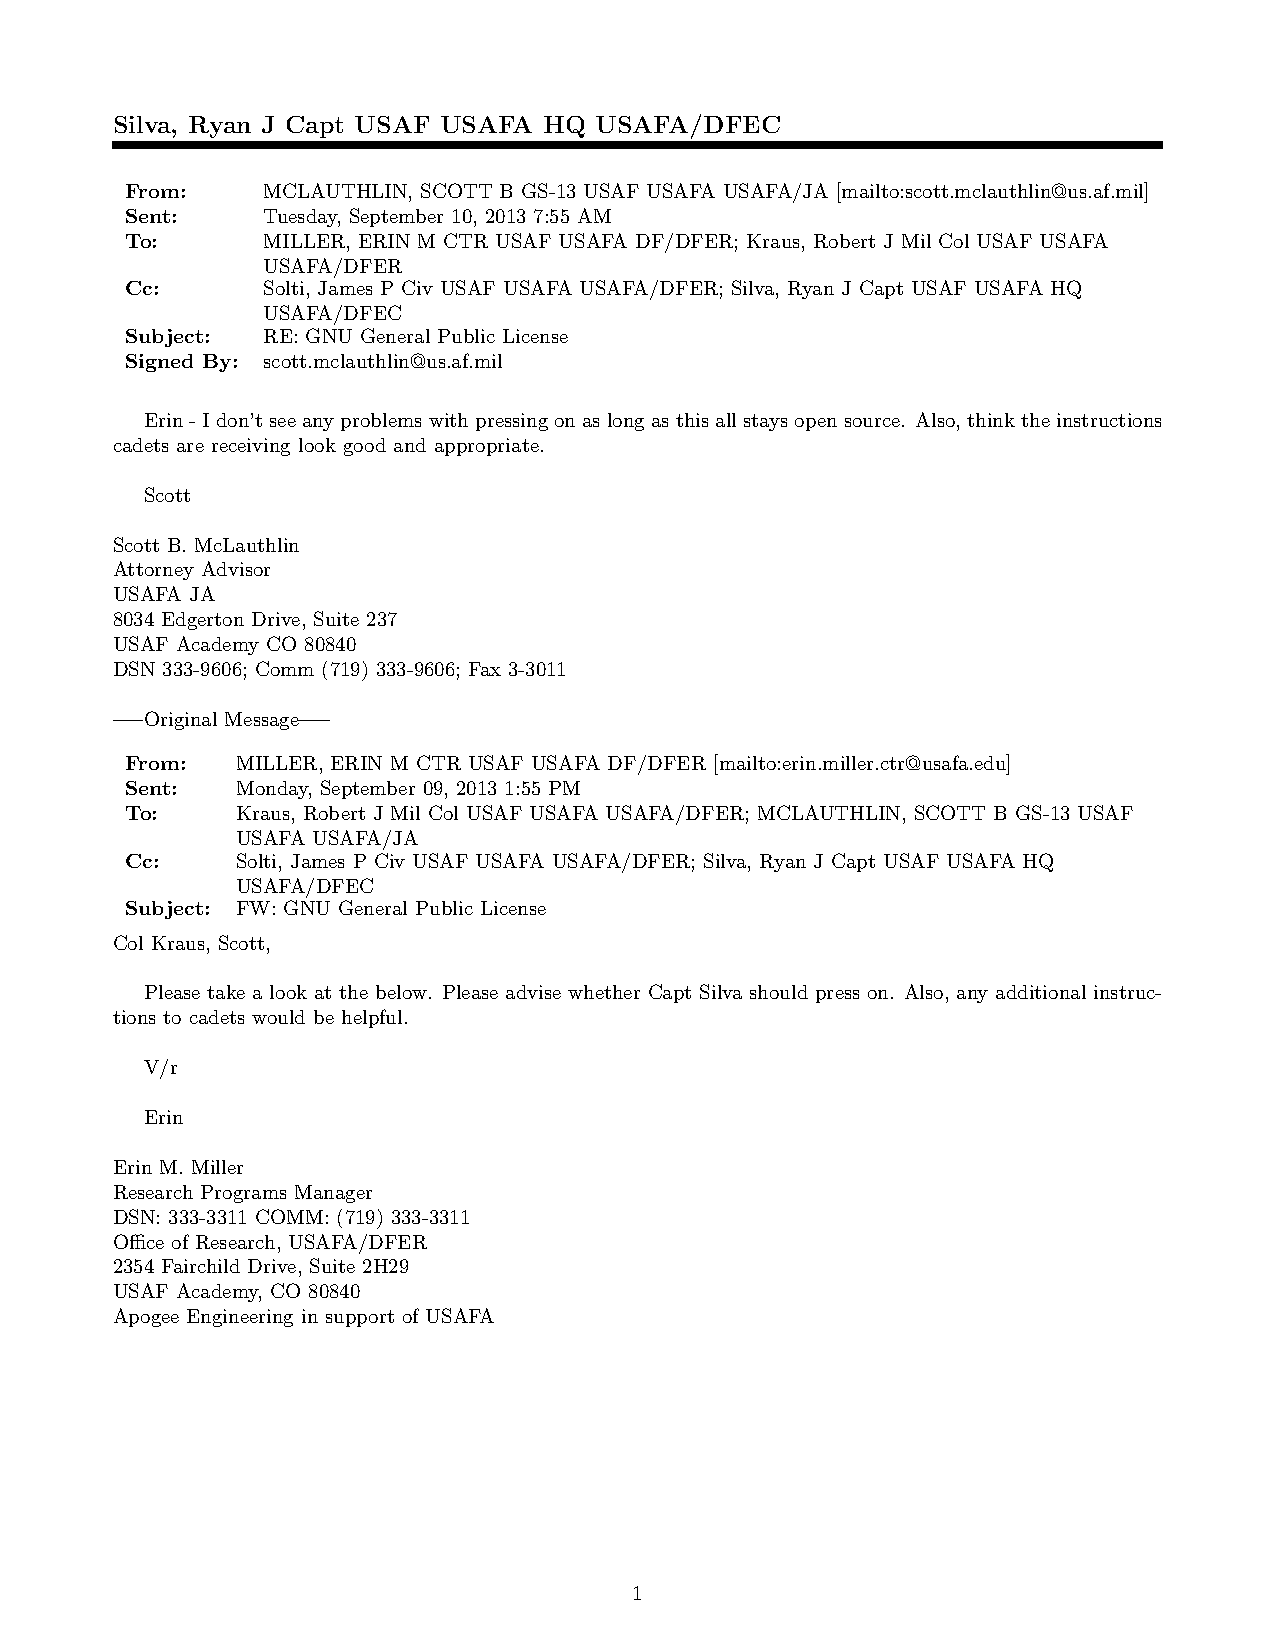
\includegraphics[scale=.85]{email.pdf}
\includepdf[pages=2,scale=0.85,offset=-0 -25,pagecommand={}]{email.pdf}
\section*{\raggedright Attachment 4 \newline May 2012 - May 2013 OPR}
\centering
\vspace{-1cm}
\hspace*{-1.5cm}
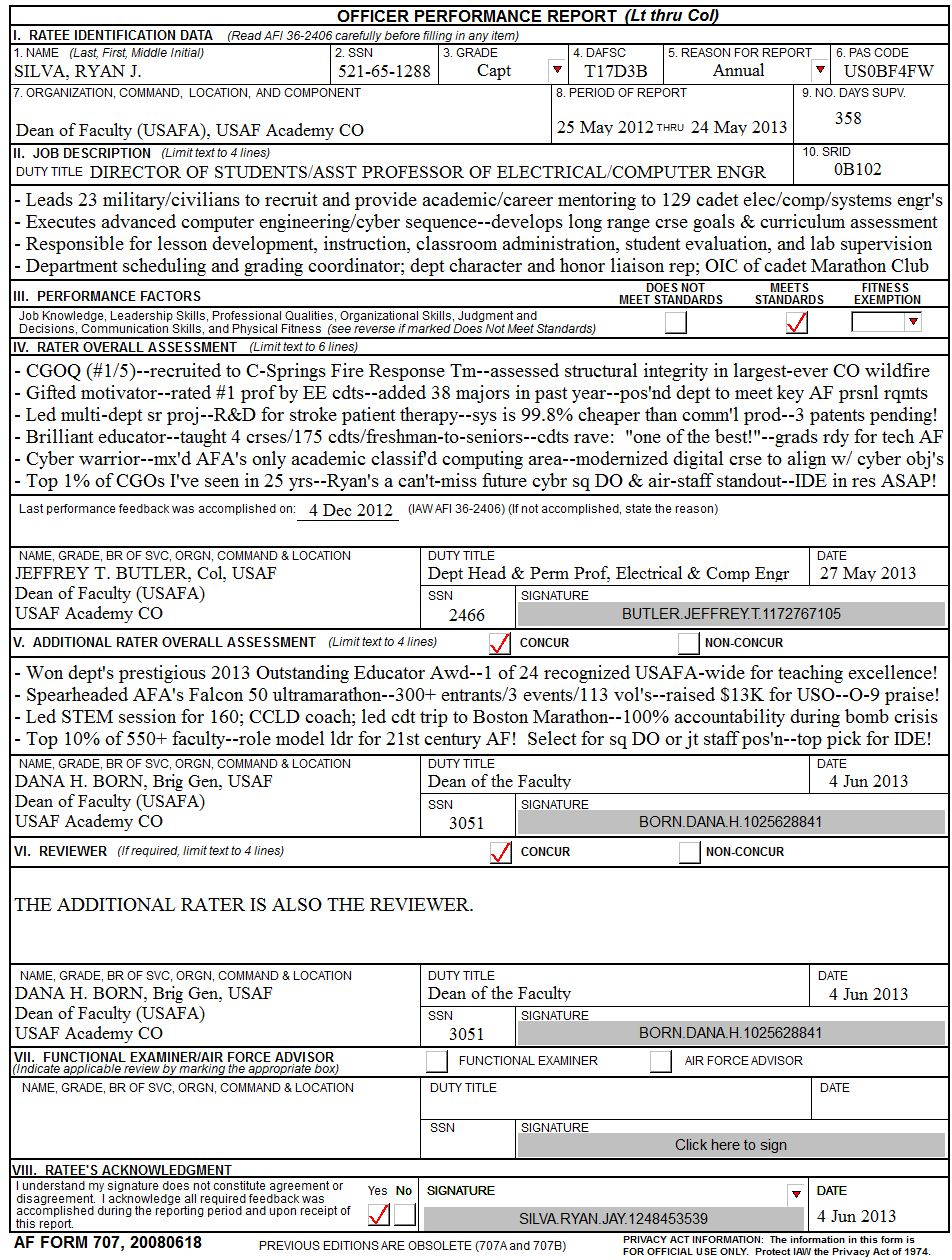
\includegraphics[scale=.65]{OPR2012-2013f}
%\label{sec:JA}

%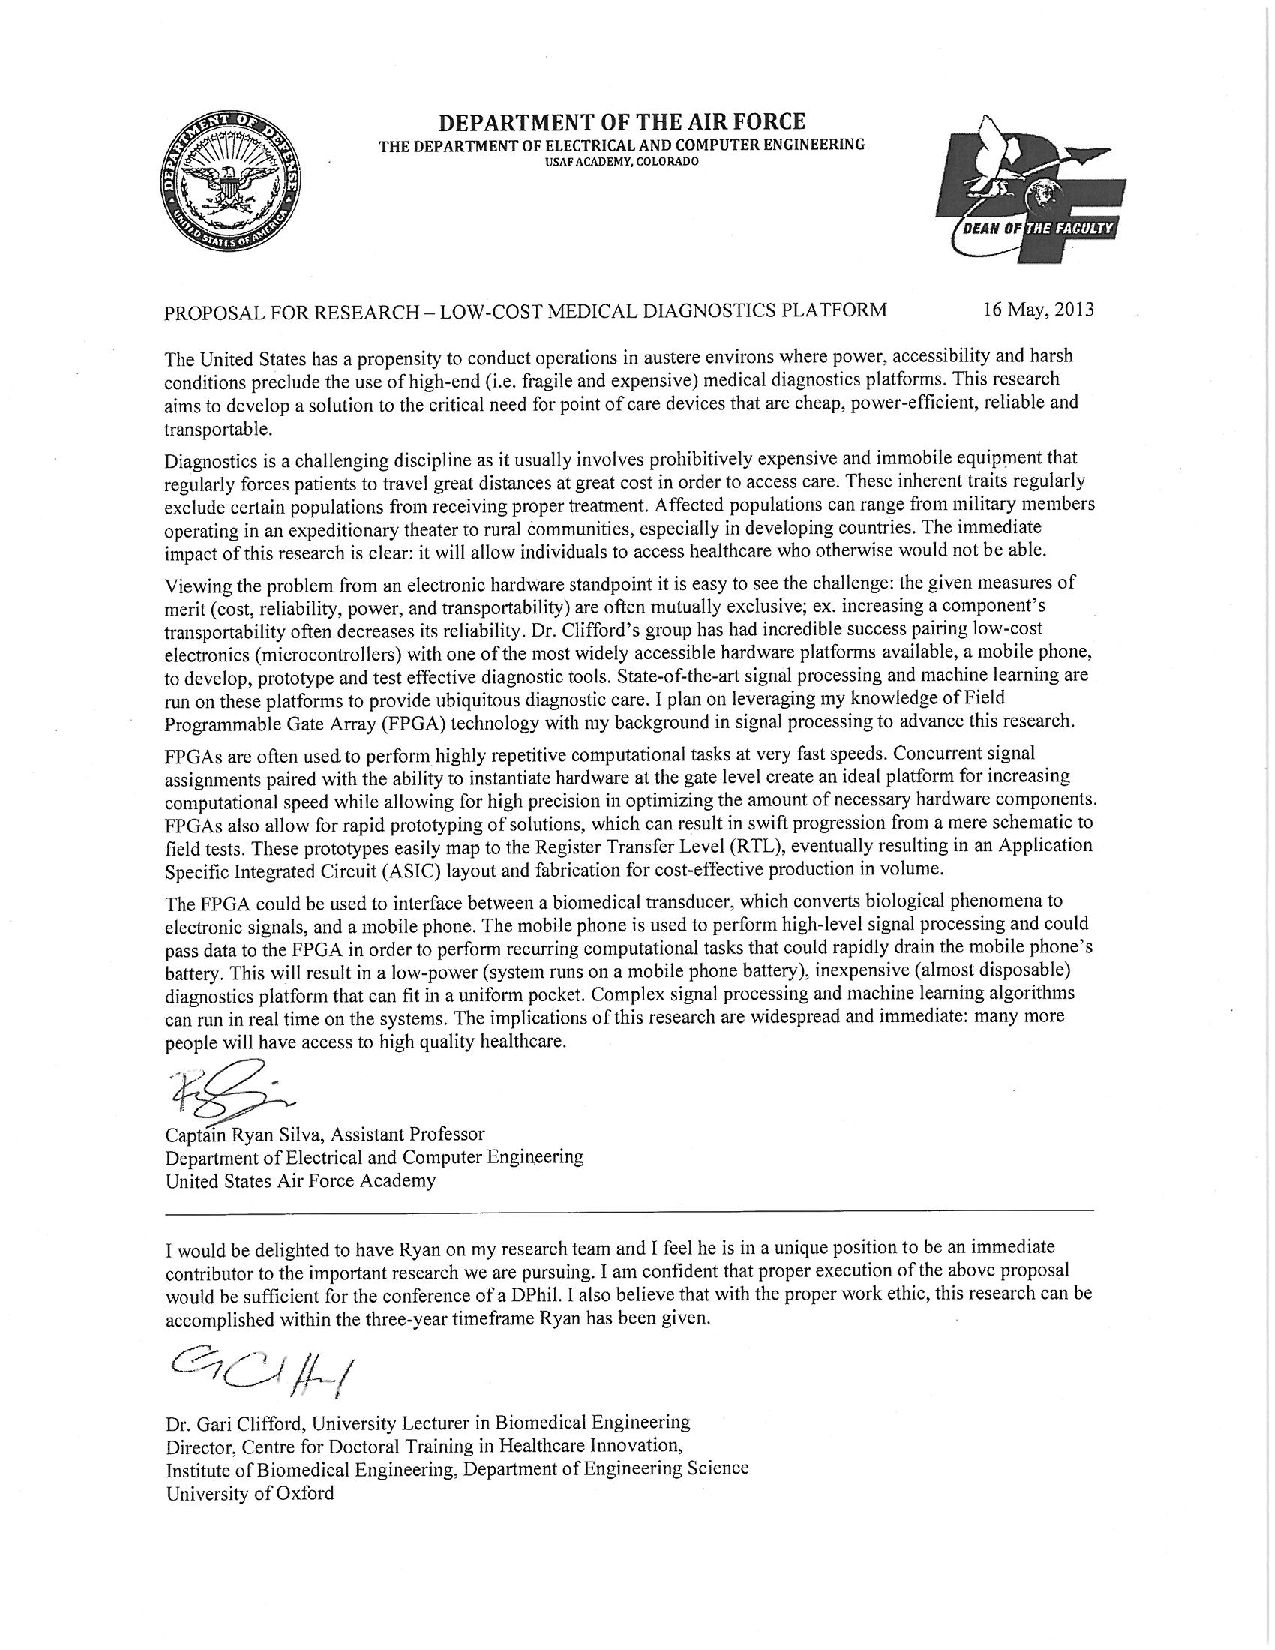
\includepdf[scale=0.8,offset=-25 -25,pagecommand={\section{Attachment - Approved Oxford Research Proposal}\label{sec:prop}}]{MFR_ProposalforResearch_SilvaSIGNED.pdf}

\end{document}
